% Created by tikzDevice version 0.8.1 on 2015-03-26 17:23:57
% !TEX encoding = UTF-8 Unicode
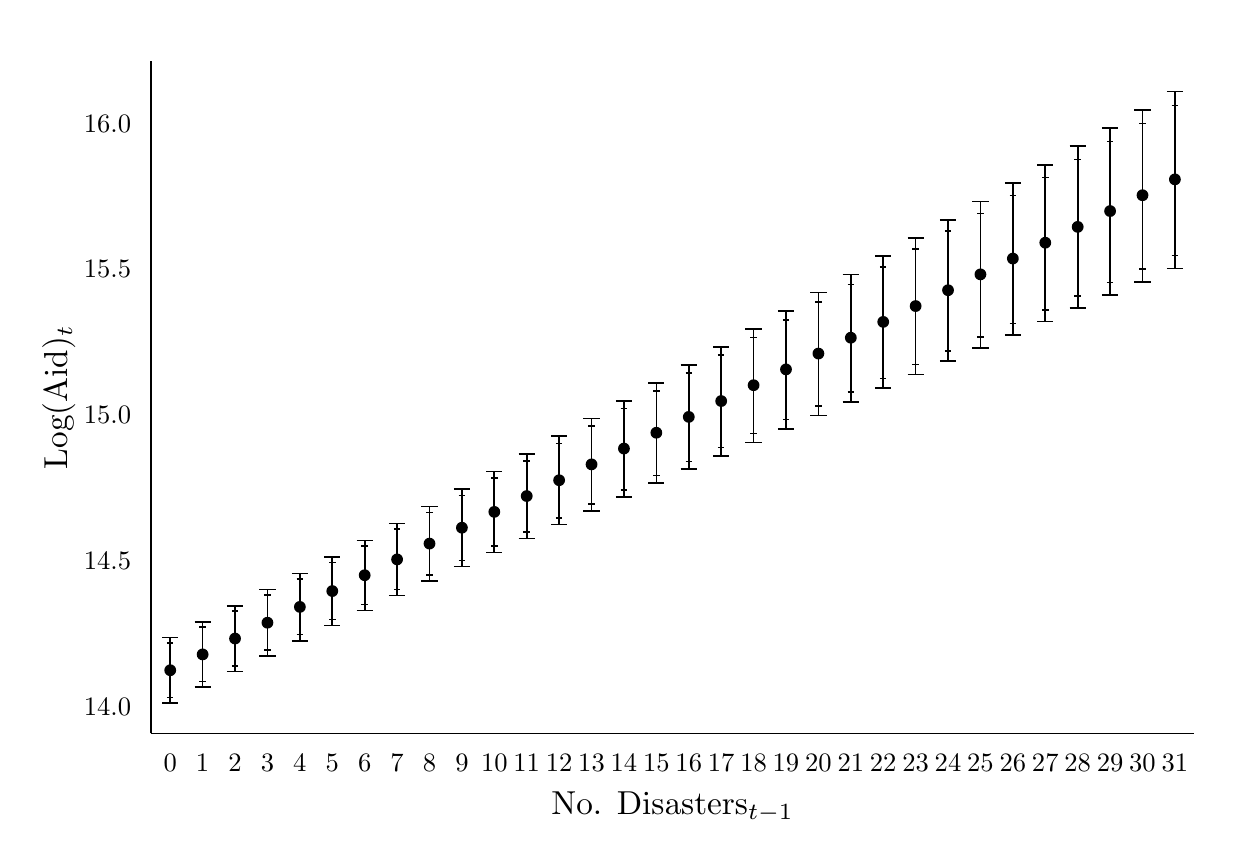
\begin{tikzpicture}[x=1pt,y=1pt]
\definecolor{fillColor}{RGB}{255,255,255}
\path[use as bounding box,fill=fillColor,fill opacity=0.00] (0,0) rectangle (433.62,289.08);
\begin{scope}
\path[clip] (  0.00,  0.00) rectangle (433.62,289.08);
\definecolor{drawColor}{RGB}{255,255,255}
\definecolor{fillColor}{RGB}{255,255,255}

\path[draw=drawColor,line width= 0.6pt,line join=round,line cap=round,fill=fillColor] (  0.00,  0.00) rectangle (433.62,289.08);
\end{scope}
\begin{scope}
\path[clip] ( 44.49, 34.03) rectangle (421.57,277.03);
\definecolor{fillColor}{RGB}{255,255,255}

\path[fill=fillColor] ( 44.49, 34.03) rectangle (421.57,277.03);
\definecolor{drawColor}{RGB}{0,0,0}

\path[draw=drawColor,line width= 0.6pt,line join=round] ( 50.34, 66.81) --
	( 52.68, 66.81);

\path[draw=drawColor,line width= 0.6pt,line join=round] ( 51.51, 66.81) --
	( 51.51, 47.00);

\path[draw=drawColor,line width= 0.6pt,line join=round] ( 50.34, 47.00) --
	( 52.68, 47.00);

\path[draw=drawColor,line width= 0.6pt,line join=round] ( 62.05, 72.43) --
	( 64.39, 72.43);

\path[draw=drawColor,line width= 0.6pt,line join=round] ( 63.22, 72.43) --
	( 63.22, 52.78);

\path[draw=drawColor,line width= 0.6pt,line join=round] ( 62.05, 52.78) --
	( 64.39, 52.78);

\path[draw=drawColor,line width= 0.6pt,line join=round] ( 73.76, 78.20) --
	( 76.10, 78.20);

\path[draw=drawColor,line width= 0.6pt,line join=round] ( 74.93, 78.20) --
	( 74.93, 58.53);

\path[draw=drawColor,line width= 0.6pt,line join=round] ( 73.76, 58.53) --
	( 76.10, 58.53);

\path[draw=drawColor,line width= 0.6pt,line join=round] ( 85.47, 84.00) --
	( 87.82, 84.00);

\path[draw=drawColor,line width= 0.6pt,line join=round] ( 86.64, 84.00) --
	( 86.64, 64.13);

\path[draw=drawColor,line width= 0.6pt,line join=round] ( 85.47, 64.13) --
	( 87.82, 64.13);

\path[draw=drawColor,line width= 0.6pt,line join=round] ( 97.18, 89.84) --
	( 99.53, 89.84);

\path[draw=drawColor,line width= 0.6pt,line join=round] ( 98.36, 89.84) --
	( 98.36, 69.77);

\path[draw=drawColor,line width= 0.6pt,line join=round] ( 97.18, 69.77) --
	( 99.53, 69.77);

\path[draw=drawColor,line width= 0.6pt,line join=round] (108.90, 95.80) --
	(111.24, 95.80);

\path[draw=drawColor,line width= 0.6pt,line join=round] (110.07, 95.80) --
	(110.07, 75.27);

\path[draw=drawColor,line width= 0.6pt,line join=round] (108.90, 75.27) --
	(111.24, 75.27);

\path[draw=drawColor,line width= 0.6pt,line join=round] (120.61,101.80) --
	(122.95,101.80);

\path[draw=drawColor,line width= 0.6pt,line join=round] (121.78,101.80) --
	(121.78, 80.62);

\path[draw=drawColor,line width= 0.6pt,line join=round] (120.61, 80.62) --
	(122.95, 80.62);

\path[draw=drawColor,line width= 0.6pt,line join=round] (132.32,107.83) --
	(134.66,107.83);

\path[draw=drawColor,line width= 0.6pt,line join=round] (133.49,107.83) --
	(133.49, 86.02);

\path[draw=drawColor,line width= 0.6pt,line join=round] (132.32, 86.02) --
	(134.66, 86.02);

\path[draw=drawColor,line width= 0.6pt,line join=round] (144.03,113.93) --
	(146.37,113.93);

\path[draw=drawColor,line width= 0.6pt,line join=round] (145.20,113.93) --
	(145.20, 91.29);

\path[draw=drawColor,line width= 0.6pt,line join=round] (144.03, 91.29) --
	(146.37, 91.29);

\path[draw=drawColor,line width= 0.6pt,line join=round] (155.74,120.06) --
	(158.08,120.06);

\path[draw=drawColor,line width= 0.6pt,line join=round] (156.91,120.06) --
	(156.91, 96.54);

\path[draw=drawColor,line width= 0.6pt,line join=round] (155.74, 96.54) --
	(158.08, 96.54);

\path[draw=drawColor,line width= 0.6pt,line join=round] (167.45,126.31) --
	(169.79,126.31);

\path[draw=drawColor,line width= 0.6pt,line join=round] (168.62,126.31) --
	(168.62,101.72);

\path[draw=drawColor,line width= 0.6pt,line join=round] (167.45,101.72) --
	(169.79,101.72);

\path[draw=drawColor,line width= 0.6pt,line join=round] (179.16,132.51) --
	(181.50,132.51);

\path[draw=drawColor,line width= 0.6pt,line join=round] (180.33,132.51) --
	(180.33,106.84);

\path[draw=drawColor,line width= 0.6pt,line join=round] (179.16,106.84) --
	(181.50,106.84);

\path[draw=drawColor,line width= 0.6pt,line join=round] (190.87,138.77) --
	(193.21,138.77);

\path[draw=drawColor,line width= 0.6pt,line join=round] (192.04,138.77) --
	(192.04,111.94);

\path[draw=drawColor,line width= 0.6pt,line join=round] (190.87,111.94) --
	(193.21,111.94);

\path[draw=drawColor,line width= 0.6pt,line join=round] (202.58,145.12) --
	(204.92,145.12);

\path[draw=drawColor,line width= 0.6pt,line join=round] (203.75,145.12) --
	(203.75,117.06);

\path[draw=drawColor,line width= 0.6pt,line join=round] (202.58,117.06) --
	(204.92,117.06);

\path[draw=drawColor,line width= 0.6pt,line join=round] (214.29,151.46) --
	(216.64,151.46);

\path[draw=drawColor,line width= 0.6pt,line join=round] (215.46,151.46) --
	(215.46,122.11);

\path[draw=drawColor,line width= 0.6pt,line join=round] (214.29,122.11) --
	(216.64,122.11);

\path[draw=drawColor,line width= 0.6pt,line join=round] (226.00,157.84) --
	(228.35,157.84);

\path[draw=drawColor,line width= 0.6pt,line join=round] (227.17,157.84) --
	(227.17,127.25);

\path[draw=drawColor,line width= 0.6pt,line join=round] (226.00,127.25) --
	(228.35,127.25);

\path[draw=drawColor,line width= 0.6pt,line join=round] (237.71,164.26) --
	(240.06,164.26);

\path[draw=drawColor,line width= 0.6pt,line join=round] (238.89,164.26) --
	(238.89,132.31);

\path[draw=drawColor,line width= 0.6pt,line join=round] (237.71,132.31) --
	(240.06,132.31);

\path[draw=drawColor,line width= 0.6pt,line join=round] (249.43,170.69) --
	(251.77,170.69);

\path[draw=drawColor,line width= 0.6pt,line join=round] (250.60,170.69) --
	(250.60,137.43);

\path[draw=drawColor,line width= 0.6pt,line join=round] (249.43,137.43) --
	(251.77,137.43);

\path[draw=drawColor,line width= 0.6pt,line join=round] (261.14,177.11) --
	(263.48,177.11);

\path[draw=drawColor,line width= 0.6pt,line join=round] (262.31,177.11) --
	(262.31,142.42);

\path[draw=drawColor,line width= 0.6pt,line join=round] (261.14,142.42) --
	(263.48,142.42);

\path[draw=drawColor,line width= 0.6pt,line join=round] (272.85,183.51) --
	(275.19,183.51);

\path[draw=drawColor,line width= 0.6pt,line join=round] (274.02,183.51) --
	(274.02,147.47);

\path[draw=drawColor,line width= 0.6pt,line join=round] (272.85,147.47) --
	(275.19,147.47);

\path[draw=drawColor,line width= 0.6pt,line join=round] (284.56,189.85) --
	(286.90,189.85);

\path[draw=drawColor,line width= 0.6pt,line join=round] (285.73,189.85) --
	(285.73,152.44);

\path[draw=drawColor,line width= 0.6pt,line join=round] (284.56,152.44) --
	(286.90,152.44);

\path[draw=drawColor,line width= 0.6pt,line join=round] (296.27,196.31) --
	(298.61,196.31);

\path[draw=drawColor,line width= 0.6pt,line join=round] (297.44,196.31) --
	(297.44,157.38);

\path[draw=drawColor,line width= 0.6pt,line join=round] (296.27,157.38) --
	(298.61,157.38);

\path[draw=drawColor,line width= 0.6pt,line join=round] (307.98,202.71) --
	(310.32,202.71);

\path[draw=drawColor,line width= 0.6pt,line join=round] (309.15,202.71) --
	(309.15,162.35);

\path[draw=drawColor,line width= 0.6pt,line join=round] (307.98,162.35) --
	(310.32,162.35);

\path[draw=drawColor,line width= 0.6pt,line join=round] (319.69,209.08) --
	(322.03,209.08);

\path[draw=drawColor,line width= 0.6pt,line join=round] (320.86,209.08) --
	(320.86,167.32);

\path[draw=drawColor,line width= 0.6pt,line join=round] (319.69,167.32) --
	(322.03,167.32);

\path[draw=drawColor,line width= 0.6pt,line join=round] (331.40,215.50) --
	(333.74,215.50);

\path[draw=drawColor,line width= 0.6pt,line join=round] (332.57,215.50) --
	(332.57,172.31);

\path[draw=drawColor,line width= 0.6pt,line join=round] (331.40,172.31) --
	(333.74,172.31);

\path[draw=drawColor,line width= 0.6pt,line join=round] (343.11,221.96) --
	(345.45,221.96);

\path[draw=drawColor,line width= 0.6pt,line join=round] (344.28,221.96) --
	(344.28,177.20);

\path[draw=drawColor,line width= 0.6pt,line join=round] (343.11,177.20) --
	(345.45,177.20);

\path[draw=drawColor,line width= 0.6pt,line join=round] (354.82,228.41) --
	(357.17,228.41);

\path[draw=drawColor,line width= 0.6pt,line join=round] (355.99,228.41) --
	(355.99,182.16);

\path[draw=drawColor,line width= 0.6pt,line join=round] (354.82,182.16) --
	(357.17,182.16);

\path[draw=drawColor,line width= 0.6pt,line join=round] (366.53,234.94) --
	(368.88,234.94);

\path[draw=drawColor,line width= 0.6pt,line join=round] (367.71,234.94) --
	(367.71,187.06);

\path[draw=drawColor,line width= 0.6pt,line join=round] (366.53,187.06) --
	(368.88,187.06);

\path[draw=drawColor,line width= 0.6pt,line join=round] (378.24,241.43) --
	(380.59,241.43);

\path[draw=drawColor,line width= 0.6pt,line join=round] (379.42,241.43) --
	(379.42,192.06);

\path[draw=drawColor,line width= 0.6pt,line join=round] (378.24,192.06) --
	(380.59,192.06);

\path[draw=drawColor,line width= 0.6pt,line join=round] (389.96,247.91) --
	(392.30,247.91);

\path[draw=drawColor,line width= 0.6pt,line join=round] (391.13,247.91) --
	(391.13,197.01);

\path[draw=drawColor,line width= 0.6pt,line join=round] (389.96,197.01) --
	(392.30,197.01);

\path[draw=drawColor,line width= 0.6pt,line join=round] (401.67,254.40) --
	(404.01,254.40);

\path[draw=drawColor,line width= 0.6pt,line join=round] (402.84,254.40) --
	(402.84,201.88);

\path[draw=drawColor,line width= 0.6pt,line join=round] (401.67,201.88) --
	(404.01,201.88);

\path[draw=drawColor,line width= 0.6pt,line join=round] (413.38,260.94) --
	(415.72,260.94);

\path[draw=drawColor,line width= 0.6pt,line join=round] (414.55,260.94) --
	(414.55,206.77);

\path[draw=drawColor,line width= 0.6pt,line join=round] (413.38,206.77) --
	(415.72,206.77);

\path[draw=drawColor,line width= 0.6pt,line join=round] ( 48.58, 68.70) --
	( 54.44, 68.70);

\path[draw=drawColor,line width= 0.6pt,line join=round] ( 51.51, 68.70) --
	( 51.51, 45.08);

\path[draw=drawColor,line width= 0.6pt,line join=round] ( 48.58, 45.08) --
	( 54.44, 45.08);

\path[draw=drawColor,line width= 0.6pt,line join=round] ( 60.30, 74.33) --
	( 66.15, 74.33);

\path[draw=drawColor,line width= 0.6pt,line join=round] ( 63.22, 74.33) --
	( 63.22, 50.83);

\path[draw=drawColor,line width= 0.6pt,line join=round] ( 60.30, 50.83) --
	( 66.15, 50.83);

\path[draw=drawColor,line width= 0.6pt,line join=round] ( 72.01, 80.15) --
	( 77.86, 80.15);

\path[draw=drawColor,line width= 0.6pt,line join=round] ( 74.93, 80.15) --
	( 74.93, 56.49);

\path[draw=drawColor,line width= 0.6pt,line join=round] ( 72.01, 56.49) --
	( 77.86, 56.49);

\path[draw=drawColor,line width= 0.6pt,line join=round] ( 83.72, 86.02) --
	( 89.57, 86.02);

\path[draw=drawColor,line width= 0.6pt,line join=round] ( 86.64, 86.02) --
	( 86.64, 62.04);

\path[draw=drawColor,line width= 0.6pt,line join=round] ( 83.72, 62.04) --
	( 89.57, 62.04);

\path[draw=drawColor,line width= 0.6pt,line join=round] ( 95.43, 91.88) --
	(101.28, 91.88);

\path[draw=drawColor,line width= 0.6pt,line join=round] ( 98.36, 91.88) --
	( 98.36, 67.56);

\path[draw=drawColor,line width= 0.6pt,line join=round] ( 95.43, 67.56) --
	(101.28, 67.56);

\path[draw=drawColor,line width= 0.6pt,line join=round] (107.14, 97.83) --
	(112.99, 97.83);

\path[draw=drawColor,line width= 0.6pt,line join=round] (110.07, 97.83) --
	(110.07, 73.07);

\path[draw=drawColor,line width= 0.6pt,line join=round] (107.14, 73.07) --
	(112.99, 73.07);

\path[draw=drawColor,line width= 0.6pt,line join=round] (118.85,103.81) --
	(124.70,103.81);

\path[draw=drawColor,line width= 0.6pt,line join=round] (121.78,103.81) --
	(121.78, 78.51);

\path[draw=drawColor,line width= 0.6pt,line join=round] (118.85, 78.51) --
	(124.70, 78.51);

\path[draw=drawColor,line width= 0.6pt,line join=round] (130.56,109.88) --
	(136.42,109.88);

\path[draw=drawColor,line width= 0.6pt,line join=round] (133.49,109.88) --
	(133.49, 83.92);

\path[draw=drawColor,line width= 0.6pt,line join=round] (130.56, 83.92) --
	(136.42, 83.92);

\path[draw=drawColor,line width= 0.6pt,line join=round] (142.27,116.06) --
	(148.13,116.06);

\path[draw=drawColor,line width= 0.6pt,line join=round] (145.20,116.06) --
	(145.20, 89.20);

\path[draw=drawColor,line width= 0.6pt,line join=round] (142.27, 89.20) --
	(148.13, 89.20);

\path[draw=drawColor,line width= 0.6pt,line join=round] (153.98,122.35) --
	(159.84,122.35);

\path[draw=drawColor,line width= 0.6pt,line join=round] (156.91,122.35) --
	(156.91, 94.34);

\path[draw=drawColor,line width= 0.6pt,line join=round] (153.98, 94.34) --
	(159.84, 94.34);

\path[draw=drawColor,line width= 0.6pt,line join=round] (165.69,128.73) --
	(171.55,128.73);

\path[draw=drawColor,line width= 0.6pt,line join=round] (168.62,128.73) --
	(168.62, 99.40);

\path[draw=drawColor,line width= 0.6pt,line join=round] (165.69, 99.40) --
	(171.55, 99.40);

\path[draw=drawColor,line width= 0.6pt,line join=round] (177.40,135.10) --
	(183.26,135.10);

\path[draw=drawColor,line width= 0.6pt,line join=round] (180.33,135.10) --
	(180.33,104.46);

\path[draw=drawColor,line width= 0.6pt,line join=round] (177.40,104.46) --
	(183.26,104.46);

\path[draw=drawColor,line width= 0.6pt,line join=round] (189.11,141.45) --
	(194.97,141.45);

\path[draw=drawColor,line width= 0.6pt,line join=round] (192.04,141.45) --
	(192.04,109.52);

\path[draw=drawColor,line width= 0.6pt,line join=round] (189.11,109.52) --
	(194.97,109.52);

\path[draw=drawColor,line width= 0.6pt,line join=round] (200.83,147.81) --
	(206.68,147.81);

\path[draw=drawColor,line width= 0.6pt,line join=round] (203.75,147.81) --
	(203.75,114.50);

\path[draw=drawColor,line width= 0.6pt,line join=round] (200.83,114.50) --
	(206.68,114.50);

\path[draw=drawColor,line width= 0.6pt,line join=round] (212.54,154.22) --
	(218.39,154.22);

\path[draw=drawColor,line width= 0.6pt,line join=round] (215.46,154.22) --
	(215.46,119.55);

\path[draw=drawColor,line width= 0.6pt,line join=round] (212.54,119.55) --
	(218.39,119.55);

\path[draw=drawColor,line width= 0.6pt,line join=round] (224.25,160.74) --
	(230.10,160.74);

\path[draw=drawColor,line width= 0.6pt,line join=round] (227.17,160.74) --
	(227.17,124.54);

\path[draw=drawColor,line width= 0.6pt,line join=round] (224.25,124.54) --
	(230.10,124.54);

\path[draw=drawColor,line width= 0.6pt,line join=round] (235.96,167.20) --
	(241.81,167.20);

\path[draw=drawColor,line width= 0.6pt,line join=round] (238.89,167.20) --
	(238.89,129.50);

\path[draw=drawColor,line width= 0.6pt,line join=round] (235.96,129.50) --
	(241.81,129.50);

\path[draw=drawColor,line width= 0.6pt,line join=round] (247.67,173.73) --
	(253.52,173.73);

\path[draw=drawColor,line width= 0.6pt,line join=round] (250.60,173.73) --
	(250.60,134.36);

\path[draw=drawColor,line width= 0.6pt,line join=round] (247.67,134.36) --
	(253.52,134.36);

\path[draw=drawColor,line width= 0.6pt,line join=round] (259.38,180.19) --
	(265.24,180.19);

\path[draw=drawColor,line width= 0.6pt,line join=round] (262.31,180.19) --
	(262.31,139.15);

\path[draw=drawColor,line width= 0.6pt,line join=round] (259.38,139.15) --
	(265.24,139.15);

\path[draw=drawColor,line width= 0.6pt,line join=round] (271.09,186.74) --
	(276.95,186.74);

\path[draw=drawColor,line width= 0.6pt,line join=round] (274.02,186.74) --
	(274.02,144.13);

\path[draw=drawColor,line width= 0.6pt,line join=round] (271.09,144.13) --
	(276.95,144.13);

\path[draw=drawColor,line width= 0.6pt,line join=round] (282.80,193.33) --
	(288.66,193.33);

\path[draw=drawColor,line width= 0.6pt,line join=round] (285.73,193.33) --
	(285.73,148.95);

\path[draw=drawColor,line width= 0.6pt,line join=round] (282.80,148.95) --
	(288.66,148.95);

\path[draw=drawColor,line width= 0.6pt,line join=round] (294.51,199.89) --
	(300.37,199.89);

\path[draw=drawColor,line width= 0.6pt,line join=round] (297.44,199.89) --
	(297.44,153.84);

\path[draw=drawColor,line width= 0.6pt,line join=round] (294.51,153.84) --
	(300.37,153.84);

\path[draw=drawColor,line width= 0.6pt,line join=round] (306.22,206.47) --
	(312.08,206.47);

\path[draw=drawColor,line width= 0.6pt,line join=round] (309.15,206.47) --
	(309.15,158.79);

\path[draw=drawColor,line width= 0.6pt,line join=round] (306.22,158.79) --
	(312.08,158.79);

\path[draw=drawColor,line width= 0.6pt,line join=round] (317.93,213.05) --
	(323.79,213.05);

\path[draw=drawColor,line width= 0.6pt,line join=round] (320.86,213.05) --
	(320.86,163.72);

\path[draw=drawColor,line width= 0.6pt,line join=round] (317.93,163.72) --
	(323.79,163.72);

\path[draw=drawColor,line width= 0.6pt,line join=round] (329.64,219.69) --
	(335.50,219.69);

\path[draw=drawColor,line width= 0.6pt,line join=round] (332.57,219.69) --
	(332.57,168.53);

\path[draw=drawColor,line width= 0.6pt,line join=round] (329.64,168.53) --
	(335.50,168.53);

\path[draw=drawColor,line width= 0.6pt,line join=round] (341.36,226.32) --
	(347.21,226.32);

\path[draw=drawColor,line width= 0.6pt,line join=round] (344.28,226.32) --
	(344.28,173.30);

\path[draw=drawColor,line width= 0.6pt,line join=round] (341.36,173.30) --
	(347.21,173.30);

\path[draw=drawColor,line width= 0.6pt,line join=round] (353.07,232.98) --
	(358.92,232.98);

\path[draw=drawColor,line width= 0.6pt,line join=round] (355.99,232.98) --
	(355.99,178.03);

\path[draw=drawColor,line width= 0.6pt,line join=round] (353.07,178.03) --
	(358.92,178.03);

\path[draw=drawColor,line width= 0.6pt,line join=round] (364.78,239.55) --
	(370.63,239.55);

\path[draw=drawColor,line width= 0.6pt,line join=round] (367.71,239.55) --
	(367.71,182.94);

\path[draw=drawColor,line width= 0.6pt,line join=round] (364.78,182.94) --
	(370.63,182.94);

\path[draw=drawColor,line width= 0.6pt,line join=round] (376.49,246.21) --
	(382.34,246.21);

\path[draw=drawColor,line width= 0.6pt,line join=round] (379.42,246.21) --
	(379.42,187.75);

\path[draw=drawColor,line width= 0.6pt,line join=round] (376.49,187.75) --
	(382.34,187.75);

\path[draw=drawColor,line width= 0.6pt,line join=round] (388.20,252.80) --
	(394.05,252.80);

\path[draw=drawColor,line width= 0.6pt,line join=round] (391.13,252.80) --
	(391.13,192.46);

\path[draw=drawColor,line width= 0.6pt,line join=round] (388.20,192.46) --
	(394.05,192.46);

\path[draw=drawColor,line width= 0.6pt,line join=round] (399.91,259.36) --
	(405.77,259.36);

\path[draw=drawColor,line width= 0.6pt,line join=round] (402.84,259.36) --
	(402.84,197.23);

\path[draw=drawColor,line width= 0.6pt,line join=round] (399.91,197.23) --
	(405.77,197.23);

\path[draw=drawColor,line width= 0.6pt,line join=round] (411.62,265.99) --
	(417.48,265.99);

\path[draw=drawColor,line width= 0.6pt,line join=round] (414.55,265.99) --
	(414.55,202.02);

\path[draw=drawColor,line width= 0.6pt,line join=round] (411.62,202.02) --
	(417.48,202.02);
\definecolor{fillColor}{RGB}{0,0,0}

\path[fill=fillColor] ( 51.51, 56.89) circle (  2.13);

\path[fill=fillColor] ( 63.22, 62.61) circle (  2.13);

\path[fill=fillColor] ( 74.93, 68.34) circle (  2.13);

\path[fill=fillColor] ( 86.64, 74.06) circle (  2.13);

\path[fill=fillColor] ( 98.36, 79.78) circle (  2.13);

\path[fill=fillColor] (110.07, 85.50) circle (  2.13);

\path[fill=fillColor] (121.78, 91.22) circle (  2.13);

\path[fill=fillColor] (133.49, 96.94) circle (  2.13);

\path[fill=fillColor] (145.20,102.66) circle (  2.13);

\path[fill=fillColor] (156.91,108.39) circle (  2.13);

\path[fill=fillColor] (168.62,114.11) circle (  2.13);

\path[fill=fillColor] (180.33,119.83) circle (  2.13);

\path[fill=fillColor] (192.04,125.55) circle (  2.13);

\path[fill=fillColor] (203.75,131.27) circle (  2.13);

\path[fill=fillColor] (215.46,136.99) circle (  2.13);

\path[fill=fillColor] (227.17,142.71) circle (  2.13);

\path[fill=fillColor] (238.89,148.43) circle (  2.13);

\path[fill=fillColor] (250.60,154.16) circle (  2.13);

\path[fill=fillColor] (262.31,159.88) circle (  2.13);

\path[fill=fillColor] (274.02,165.60) circle (  2.13);

\path[fill=fillColor] (285.73,171.32) circle (  2.13);

\path[fill=fillColor] (297.44,177.04) circle (  2.13);

\path[fill=fillColor] (309.15,182.76) circle (  2.13);

\path[fill=fillColor] (320.86,188.48) circle (  2.13);

\path[fill=fillColor] (332.57,194.21) circle (  2.13);

\path[fill=fillColor] (344.28,199.93) circle (  2.13);

\path[fill=fillColor] (355.99,205.65) circle (  2.13);

\path[fill=fillColor] (367.71,211.37) circle (  2.13);

\path[fill=fillColor] (379.42,217.09) circle (  2.13);

\path[fill=fillColor] (391.13,222.81) circle (  2.13);

\path[fill=fillColor] (402.84,228.53) circle (  2.13);

\path[fill=fillColor] (414.55,234.26) circle (  2.13);
\end{scope}
\begin{scope}
\path[clip] (  0.00,  0.00) rectangle (433.62,289.08);
\definecolor{drawColor}{RGB}{0,0,0}

\path[draw=drawColor,line width= 0.6pt,line join=round] ( 44.49, 34.03) --
	( 44.49,277.03);
\end{scope}
\begin{scope}
\path[clip] (  0.00,  0.00) rectangle (433.62,289.08);
\definecolor{drawColor}{RGB}{0,0,0}

\node[text=drawColor,anchor=base east,inner sep=0pt, outer sep=0pt, scale=  0.96] at ( 37.37, 40.49) {14.0};

\node[text=drawColor,anchor=base east,inner sep=0pt, outer sep=0pt, scale=  0.96] at ( 37.37, 93.22) {14.5};

\node[text=drawColor,anchor=base east,inner sep=0pt, outer sep=0pt, scale=  0.96] at ( 37.37,145.94) {15.0};

\node[text=drawColor,anchor=base east,inner sep=0pt, outer sep=0pt, scale=  0.96] at ( 37.37,198.66) {15.5};

\node[text=drawColor,anchor=base east,inner sep=0pt, outer sep=0pt, scale=  0.96] at ( 37.37,251.38) {16.0};
\end{scope}
\begin{scope}
\path[clip] (  0.00,  0.00) rectangle (433.62,289.08);
\definecolor{drawColor}{RGB}{0,0,0}

\path[draw=drawColor,line width= 0.6pt,line join=round] ( 44.49, 34.03) --
	(421.57, 34.03);
\end{scope}
\begin{scope}
\path[clip] (  0.00,  0.00) rectangle (433.62,289.08);
\definecolor{drawColor}{RGB}{0,0,0}

\node[text=drawColor,anchor=base,inner sep=0pt, outer sep=0pt, scale=  0.96] at ( 51.51, 20.31) {0};

\node[text=drawColor,anchor=base,inner sep=0pt, outer sep=0pt, scale=  0.96] at ( 63.22, 20.31) {1};

\node[text=drawColor,anchor=base,inner sep=0pt, outer sep=0pt, scale=  0.96] at ( 74.93, 20.31) {2};

\node[text=drawColor,anchor=base,inner sep=0pt, outer sep=0pt, scale=  0.96] at ( 86.64, 20.31) {3};

\node[text=drawColor,anchor=base,inner sep=0pt, outer sep=0pt, scale=  0.96] at ( 98.36, 20.31) {4};

\node[text=drawColor,anchor=base,inner sep=0pt, outer sep=0pt, scale=  0.96] at (110.07, 20.31) {5};

\node[text=drawColor,anchor=base,inner sep=0pt, outer sep=0pt, scale=  0.96] at (121.78, 20.31) {6};

\node[text=drawColor,anchor=base,inner sep=0pt, outer sep=0pt, scale=  0.96] at (133.49, 20.31) {7};

\node[text=drawColor,anchor=base,inner sep=0pt, outer sep=0pt, scale=  0.96] at (145.20, 20.31) {8};

\node[text=drawColor,anchor=base,inner sep=0pt, outer sep=0pt, scale=  0.96] at (156.91, 20.31) {9};

\node[text=drawColor,anchor=base,inner sep=0pt, outer sep=0pt, scale=  0.96] at (168.62, 20.31) {10};

\node[text=drawColor,anchor=base,inner sep=0pt, outer sep=0pt, scale=  0.96] at (180.33, 20.31) {11};

\node[text=drawColor,anchor=base,inner sep=0pt, outer sep=0pt, scale=  0.96] at (192.04, 20.31) {12};

\node[text=drawColor,anchor=base,inner sep=0pt, outer sep=0pt, scale=  0.96] at (203.75, 20.31) {13};

\node[text=drawColor,anchor=base,inner sep=0pt, outer sep=0pt, scale=  0.96] at (215.46, 20.31) {14};

\node[text=drawColor,anchor=base,inner sep=0pt, outer sep=0pt, scale=  0.96] at (227.17, 20.31) {15};

\node[text=drawColor,anchor=base,inner sep=0pt, outer sep=0pt, scale=  0.96] at (238.89, 20.31) {16};

\node[text=drawColor,anchor=base,inner sep=0pt, outer sep=0pt, scale=  0.96] at (250.60, 20.31) {17};

\node[text=drawColor,anchor=base,inner sep=0pt, outer sep=0pt, scale=  0.96] at (262.31, 20.31) {18};

\node[text=drawColor,anchor=base,inner sep=0pt, outer sep=0pt, scale=  0.96] at (274.02, 20.31) {19};

\node[text=drawColor,anchor=base,inner sep=0pt, outer sep=0pt, scale=  0.96] at (285.73, 20.31) {20};

\node[text=drawColor,anchor=base,inner sep=0pt, outer sep=0pt, scale=  0.96] at (297.44, 20.31) {21};

\node[text=drawColor,anchor=base,inner sep=0pt, outer sep=0pt, scale=  0.96] at (309.15, 20.31) {22};

\node[text=drawColor,anchor=base,inner sep=0pt, outer sep=0pt, scale=  0.96] at (320.86, 20.31) {23};

\node[text=drawColor,anchor=base,inner sep=0pt, outer sep=0pt, scale=  0.96] at (332.57, 20.31) {24};

\node[text=drawColor,anchor=base,inner sep=0pt, outer sep=0pt, scale=  0.96] at (344.28, 20.31) {25};

\node[text=drawColor,anchor=base,inner sep=0pt, outer sep=0pt, scale=  0.96] at (355.99, 20.31) {26};

\node[text=drawColor,anchor=base,inner sep=0pt, outer sep=0pt, scale=  0.96] at (367.71, 20.31) {27};

\node[text=drawColor,anchor=base,inner sep=0pt, outer sep=0pt, scale=  0.96] at (379.42, 20.31) {28};

\node[text=drawColor,anchor=base,inner sep=0pt, outer sep=0pt, scale=  0.96] at (391.13, 20.31) {29};

\node[text=drawColor,anchor=base,inner sep=0pt, outer sep=0pt, scale=  0.96] at (402.84, 20.31) {30};

\node[text=drawColor,anchor=base,inner sep=0pt, outer sep=0pt, scale=  0.96] at (414.55, 20.31) {31};
\end{scope}
\begin{scope}
\path[clip] (  0.00,  0.00) rectangle (433.62,289.08);
\definecolor{drawColor}{RGB}{0,0,0}

\node[text=drawColor,anchor=base,inner sep=0pt, outer sep=0pt, scale=  1.20] at (233.03,  4.82) {No. Disasters$_{t-1}$};
\end{scope}
\begin{scope}
\path[clip] (  0.00,  0.00) rectangle (433.62,289.08);
\definecolor{drawColor}{RGB}{0,0,0}

\node[text=drawColor,rotate= 90.00,anchor=base,inner sep=0pt, outer sep=0pt, scale=  1.20] at ( 14.29,155.53) {Log(Aid)$_{t}$};
\end{scope}
\end{tikzpicture}
